\documentclass[11pt,a4paper]{article}   % 11 pt text on A4 paper

% References
\usepackage{csquotes}                   % quotation marks that follow the document's language
\usepackage[backend=biber,style=apa,natbib=true]{biblatex} % APA 7; compile with Biber
\DeclareLanguageMapping{australian}{british-apa}
\usepackage{xurl} % allow long bibliography URLs to wrap within the page
\addbibresource{references.bib}

% Page
\usepackage[margin=25mm]{geometry}      % 25 mm margins all round
\usepackage{parskip}                    % a blank line between paragraphs instead of an indent
\usepackage[australian]{babel}          % Australian hyphenation, and \today as 17 October 2026
\usepackage{iftex}                      % tells which TeX engine is running
\ifPDFTeX                               % for pdfLaTeX only:
  \usepackage[T1]{fontenc}              % proper accented letters, and text that copies cleanly from the PDF
  \usepackage{lmodern}                  % Latin Modern, a crisp scalable version of the default font
\fi                                     % XeLaTeX, LuaLaTeX and Tectonic already use Unicode fonts, which print a typed ’ or é as it is

% Maths and units
\usepackage{amsmath}                    % align, cases, matrices and \text inside maths
\usepackage{amssymb}                    % extra symbols such as \mathbb{R}
\usepackage{amsthm}                     % example and proof environments
\usepackage{siunitx}                    % \qty{4.7}{\kilo\ohm} and \unit{\hertz}; older notes use \SI, which still works
\sisetup{per-mode = symbol}             % write units as V/µs rather than V µs⁻¹

% Figures and tables
\usepackage[american]{circuitikz}       % circuit diagrams; american = zigzag resistors and +/- voltage labels
\usepackage{pgfplots}                   % plotting responses and data, built on TikZ
\pgfplotsset{compat=1.18}               % use current pgfplots behaviour (label placement and so on)
\usepackage{booktabs}                   % \toprule, \midrule and \bottomrule for clean tables
\usepackage{tabularx}                   % tables that stretch to a set width
\usepackage{graphicx}                   % \includegraphics for photos, scope captures and screenshots

% Links
\usepackage[hidelinks]{hyperref}        % clickable cross-references, without coloured boxes
\hypersetup{                            % details shown in the PDF viewer’s document properties
  pdftitle  = {Week 6: Active filters},
  pdfauthor = {Your Name},
  pdflang   = {en-AU}
}
\usepackage[capitalise,noabbrev]{cleveref} % \cref{fig:filter} writes “Figure 1.1” for you; load after hyperref

% Number equations, figures and tables by section: (1.1), Figure 1.1, ...
\numberwithin{equation}{section}
\numberwithin{figure}{section}
\numberwithin{table}{section}

% Worked examples, numbered by section, each followed by a solution
\theoremstyle{definition}               % upright text
\newtheorem{example}{Example}[section]
\newenvironment{solution}{\begin{proof}[Solution]}{\end{proof}}

\title{Week 6: Active filters}
\author{Your Name}
\date{Semester 2, 2026}

\begin{document}
\maketitle

\section{The inverting low-pass filter}

Putting a capacitor $C$ across the feedback resistor of an inverting amplifier turns it into a
first-order low-pass filter (\cref{fig:filter}). It passes low frequencies with the gain of
the amplifier and rolls off at \qty{-20}{\decibel} per decade above its cut-off frequency.

\begin{figure}[ht]
  \centering
  \begin{circuitikz}
    \draw (0,0) node[op amp] (A) {}
      (A.-) -- ++(-0.5,0) coordinate (n)
      (n) to[R, l_=$R_\mathrm{in}$, -o] ++(-3,0) node[left] {$v_\mathrm{in}$}
      (n) to[short, *-] ++(0,1.5) coordinate (r) to[R, l=$R_f$, *-*] (r -| A.out) coordinate (o)
      (r) -- ++(0,1.5) coordinate (c) to[C, l=$C$] (c -| A.out) -- (o) to[short, -*] (A.out)
      (A.+) -- ++(0,-0.5) node[ground] {}
      (A.out) to[short, -o] ++(1,0) node[right] {$v_\mathrm{out}$};
  \end{circuitikz}
  \caption{An inverting amplifier with a capacitor in its feedback path.}
  \label{fig:filter}
\end{figure}

With an ideal op-amp the inverting input is a virtual earth, so the current through
$R_\mathrm{in}$ all flows through the feedback impedance
$Z_f = R_f \parallel \frac{1}{j\omega C} = \frac{R_f}{1 + j\omega R_f C}$. Hence
\begin{equation}\label{eq:gain}
  H(j\omega) = \frac{v_\mathrm{out}}{v_\mathrm{in}} = -\frac{Z_f}{R_\mathrm{in}}
  = -\frac{R_f}{R_\mathrm{in}} \cdot \frac{1}{1 + j\omega R_f C},
\end{equation}
and the cut-off frequency, where the gain has fallen by \qty{3}{\decibel}, is
\begin{equation}\label{eq:cutoff}
  f_c = \frac{1}{2\pi R_f C}.
\end{equation}

\begin{example}\label{ex:design}
The filter in \cref{fig:filter} uses the parts in \cref{tab:parts}. Find its passband
gain in decibels and its cut-off frequency.
\end{example}

\begin{table}[ht]
  \centering
  \caption{Parts for the filter in \cref{ex:design}.}
  \label{tab:parts}
  \begin{tabularx}{0.8\textwidth}{l l X}
    \toprule
    Part & Value & Purpose \\
    \midrule
    $R_\mathrm{in}$ & \qty{4.7}{\kilo\ohm} & sets the input current \\
    $R_f$ & \qty{47}{\kilo\ohm} & sets the passband gain, with $R_\mathrm{in}$ \\
    $C$ & \qty{3.3}{\nano\farad} & rolls the gain off above $f_c$ \\
    Op-amp & TL071 & JFET-input op-amp on a \qty{\pm 15}{\volt} supply \\
    \bottomrule
  \end{tabularx}
\end{table}

\begin{solution}
At low frequencies $\omega R_f C \ll 1$, so by \cref{eq:gain} the gain is
$-R_f / R_\mathrm{in} = -47 / 4.7 = -10$, that is $20 \log_{10} 10 = \qty{20}{\decibel}$ with the
output inverted. By \cref{eq:cutoff},
\[
  f_c = \frac{1}{2\pi \times \qty{47e3}{\ohm} \times \qty{3.3e-9}{\farad}}
      \approx \qty{1.03}{\kilo\hertz}.
\]
\cref{fig:bode} plots the magnitude of \cref{eq:gain} for these values.
\end{solution}

\begin{figure}[ht]
  \centering
  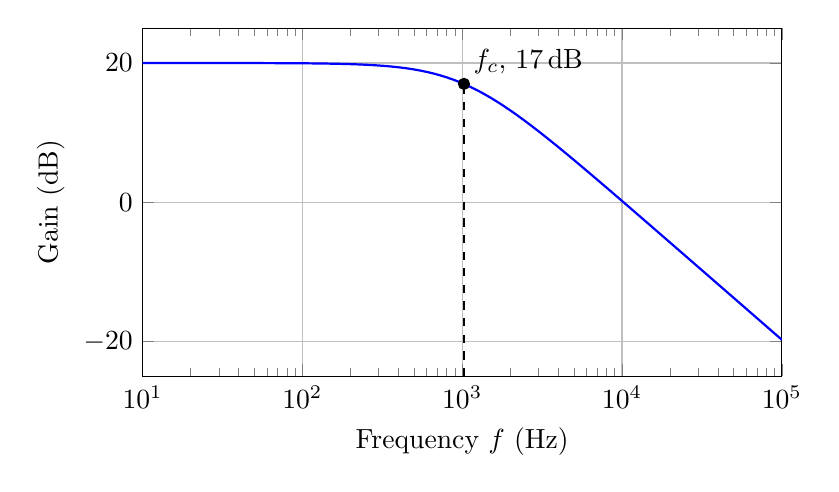
\begin{tikzpicture}
    \begin{semilogxaxis}[
        width=0.8\textwidth, height=6cm, grid=major,
        xmin=10, xmax=1e5, ymin=-25, ymax=25,
        xlabel={Frequency $f$ (\unit{\hertz})}, ylabel={Gain (\unit{\decibel})}]
      % sampled in powers of ten so the points spread evenly along the log axis
      \addplot[thick, blue, domain=1:5, samples=100]
        ({10^x}, {20 - 10*log10(1 + (10^x/1026)^2)});
      \draw[dashed] (axis cs:1026,-25) -- (axis cs:1026,17);
      \addplot[only marks, mark=*] coordinates {(1026,17)}
        node[above right] {$f_c$, \qty{17}{\decibel}};
    \end{semilogxaxis}
  \end{tikzpicture}
  \caption{Gain of the filter in \cref{ex:design}: flat at \qty{20}{\decibel}, then
    falling at \qty{20}{\decibel} per decade above $f_c$.}
  \label{fig:bode}
\end{figure}

\section{Practical limits}

A real op-amp only approximates \cref{eq:gain}. The TL071's slew rate of
\qty{13}{\volt\per\micro\second} caps how fast the output can swing, so a \qty{10}{\volt} peak
sine wave starts to distort above about
$\frac{\qty{13}{\volt\per\micro\second}}{2\pi \times \qty{10}{\volt}} \approx \qty{207}{\kilo\hertz}$,
well above this filter's cut-off.

\printbibliography

\end{document}
